% To check for overfull hboxes, add draft to the document options
\documentclass[a4paper, 10pt]{IEEEtran}
\usepackage[english]{babel}   % Taal van het document (opmaakregels ed.)
%\usepackage{fancyhdr} % Fancy headers & footers

\usepackage{graphicx}
\usepackage[tight]{subfigure}	% Multiple figures in one float

\usepackage{color}
\usepackage{colortbl}	% Use colors in table
\usepackage{multirow}	% Multiple rows and columns in tables
\usepackage{booktabs}	% Professional looking tables

\usepackage{amsmath,amsfonts}    % Wiskunde

\usepackage{listings}            % Code Listings
%\usepackage[subfigure]{tocloft}		% Lijsten van willekeurige dingen + optie om errors met subfigure te vermijden
%\usepackage{url}                % Opmaak van URLs

\usepackage[pdftex, pdfborder={0 0 0}]{hyperref}	% Links in pdf

\usepackage{algorithmic}
\usepackage{algorithm}

% Titel etc
\title{Compact implementations of pairings}
\author{Anthony Van Herrewege\thanks{Anthony Van Herrewege obtained his B.S.\ in computer engineering from K.U.\ Leuven, Leuven, Belgium in 2007. This paper is part of his thesis towards obtaining a M.Sc.\ in electrical engineering from the same university. Email: anthonyvh@gmail.com.}}
\date{22 May 2009}

% Math stuff
\newcommand{\xor}{\oplus}

% Citatie commando's
\newcommand{\reffig}[1]{Fig.~\ref{#1}}
\newcommand{\reftbl}[1]{Table~\ref{#1}}
\newcommand{\refalg}[1]{Algorithm~\ref{#1}}
\newcommand{\refsect}[1]{Section~\ref{#1}}
\newcommand{\refhfdst}[1]{Chapter~\ref{#1}}
\newcommand{\refform}[1]{Formula~\ref{#1}}

% Misc commando's
\newcommand{\nr}{n$^{\circ}$~}
%\renewcommand{\thefootnote}{\fnsymbol{footnote}}	% Voetnoten met symbolen ipv nummers

% Narrow environment for wide tables & figures
% Usage: \begin{narrow}{-left cm}{-right cm}
\newenvironment{narrow}[2]{%
  \begin{list}{}{%
    \setlength{\topsep}{0pt}%
    \setlength{\leftmargin}{#1}%
    \setlength{\rightmargin}{#2}%
    \setlength{\listparindent}{\parindent}%
    \setlength{\itemindent}{\parindent}%
    \setlength{\parsep}{\parskip}%
  }%
  \item[]
}{\end{list}}

% BibTex opmaak
\bibliographystyle{IEEEtran} % Unsorted IEEE style

% Fix for unsorted bibliographies & citations in captions
\def\@starttoc#1{%
  \begingroup
    \@fileswfalse
    \makeatletter
    \@input{\jobname.#1}%
  \endgroup
  \if@filesw
    \expandafter\newwrite\csname tf@#1\endcsname
    \immediate\openout \csname tf@#1\endcsname \jobname.#1\relax
  \fi
  \@nobreakfalse
}

% Plaats van afbeeldingen
\graphicspath{{../images/}}
\DeclareGraphicsExtensions{.pdf,.eps,.png}

% Fix caption spacing bij tabellen
%\setlength{\belowcaptionskip}{6pt}

% Regel nummering van figuren
%\renewcommand{\thefigure}{\thechapter.\arabic{figure}}
%\newcommand{\Chapter}[1]{\chapter{#1} \setcounter{figure}{0}}

\begin{document}
\selectlanguage{english}  % Set hyphenation patterns

% Include gedeelte (begint op nieuwe pagina
% Indien gewoon invoegen op huidige plaats \input

\maketitle

\begin{abstract}
The recent discovery of the constructive use of pairings in cryptography has opened up a wealth of new research options into identity-based encryption. In this paper, we will investigate the possible use of pairings in constrained environments. The focus will be on an small, energy efficient ASIC implementation of an accelerator for the Tate pairing over a supersingular curve.

The results are encouraging for further research. It is possible to obtain an implementation of less than 30k~gates consuming only 206~nA. Furthermore, energy efficiency improvements over twenty times compared to other published designs are possible.
\end{abstract}

\begin{IEEEkeywords}
Identity-based cryptography, elliptic curve cryptography, Tate pairing, hardware accelerator, ASIC.
\end{IEEEkeywords}



\section{Introduction\label{section-introduction}}

\IEEEPARstart{E}{ver} since Shamir's proposal \cite{shamir} in '84, there's been an interest in identity-based cryptography. Particularly Boneh and Franklin's \cite{boneh} discovery of the constructive use of pairings for identity-based encryption has helped spur on new research into possible applications and implementations.

Multitudes of protocols have seen the light, however, until recently the lack of efficient hardware accelerators for the computationally expensive pairings was always kind of a show-stopper towards implementing them. Thus most of the published implementations have a focus on speed. Implementations for area- and/or power-constrained devices were either deemed infeasible or just not interesting enough. 

In 2007 Oliveira \emph{et al.} introduced their TinyTate \cite{tinytate} implementation to the world. 2008 saw the light of TinyPBC \cite{tinypbc} and NanoECC \cite{nanoecc} from the same authors. All three papers present implementations of pairings (either the Tate or $\eta_T$) on the AT128Mega microchip of a Mica node \cite{mica}, designed for deeply embedded networks. Thus it was proven that pairings were indeed feasible for use in constrained environments, such as sensor networks.

In this paper, we will investigate the feasibility of a hardware accelerator for the Tate pairing in constrained environments. In \refsect{section-pairings} necessary parameters will be defined and we will take a look at the pairing arithmetic. \refsect{section-hardware} consist of a concise overview of the implementation's hardware. Finally, results from synthesis to an ASIC implementation will be presented along with comparisons to existing implementations in \refsect{section-results}. From these a conclusion will be drawn in \refsect{section-conclusion}.

\section{Parameters and arithmetic for the Tate pairing\label{section-pairings}}

As mentioned, we will be creating an accelerator for the Tate pairing. Recently, variants on that pairing have been published, such as the $\eta_T$ \cite{eta} and Ate \cite{ate} pairings. However, seeing as they are very recent discoveries, we felt it more appropriate to focus on the better known Tate pairing.

\subsection{Definition of the Tate pairing}

The Tate pairing $e(P, Q)$ is defined as a mapping from two additive groups $\mathbb{G}_1, \mathbb{G}_2$ to a multiplicative group $\mathbb{G}_T$. To be suitable for use in cryptography, it should have the following three properties:
\begin{itemize}
	\item Well-defined:%
		\begin{displaymath}\begin{aligned}
			e(\mathcal{O}, Q) &= 1 \: \forall \: Q \in \mathbb{G}_2\\
			e(P, \mathcal{O}) &= 1 \: \forall \: P \in \mathbb{G}_1.
		\end{aligned}\end{displaymath}
	
	\item Non-degenerate:%
		\begin{displaymath}\forall \: P \in \mathbb{G}_1, \: \exists \: Q \in \mathbb{G}_2 \text{ for which } e(P, Q) \neq 1.\end{displaymath}
	
	\item Bilinear: $\forall \: P_1, P_2, P \in \mathbb{G}_1$ and $\forall \: Q_1, Q_2, Q \in \mathbb{G}_2$:%
		\begin{displaymath}\begin{aligned}
			e(P_1 + P_2, Q) &\equiv e(P_1, Q) \cdot e(P_2, Q)\\
			e(P, Q_1 + Q_2) &\equiv e(P, Q_1) \cdot e(P, Q_2).
		\end{aligned}\end{displaymath}
\end{itemize}
The point $\mathcal{O}$ is the point at infinity on the elliptic curve $E$ over which the pairing is defined.

Instead of calculating the Tate pairing as proposed by Miller in '86 \cite{miller}, we will be using an optimized version of Miller's algorithm as proposed by Barreto \emph{et al.} \cite{barreto-efficient}. The Tate pairing is then a mapping:
\begin{displaymath}
\hat{e}(P, Q) : E(\mathbb{F}_q) [l] \times E(\mathbb{F}_q) [l] \mapsto \mathbb{F}_{q^k}^*/(\mathbb{F}_{q^k}^*)^l.
\end{displaymath}
The notation $E(\mathbb{F}_q) [l]$ meaning the group of points $P \in E(\mathbb{F}_q)$ for which $l P = \mathcal{O}$. The result of the pairing is an element of the equivalence group $\mathbb{F}_{q^k}^*/(\mathbb{F}_{q^k}^*)^l$, in which two elements $a \equiv b$ iif $a = bc^l$ with $c \in \mathbb{F}_{q^k}^*$. To eliminate this ambiguity, we will elevate the result of the pairing to the power $\frac{q^k - 1}{l}$, the result of which will be an $l$th root of unity $\mu_l$.

\subsection{Parameters}

Before we can take a look at the arithmetic behind the Tate pairing computation, some parameters need to be set. First and foremost, the elliptic curve and the field over which it is defined need to be defined. Due to the simplicity of its arithmetic (only XORing), we choose a field $\mathbb{F}_{2^m}$. We are then forced to use the curve \cite{barreto-efficient}:
\begin{displaymath}
E(\mathbb{F}_{2^m}) : y^3 + y = x^3 + x + b,
\end{displaymath}
with $b \in \{0,1\}$. We also define \cite{beuchat}:
\begin{displaymath}\begin{aligned}
\delta	&= \begin{cases}
				b		\qquad &m \equiv 1, 7 \pmod 8\\
				1 - b			&m \equiv 3, 5	\pmod 8
				\end{cases}\\
\nu		&= (-1)^{\delta}
\end{aligned}\end{displaymath}
The value of $b$ set to whatever value maximizes the order of the curve:
\begin{displaymath}
\#E(\mathbb{F}_{2^m}) = 2^m + \nu \sqrt{2^{m+1}} + 1.
\end{displaymath}
So, before the value of $b$ can be decided on, $m$ is to be set. We also define $l = \#E$.

Considering that the final implementation should be as small as possible, we settle on $m = 163$, which, according to \cite{lenstra}, should still provide reasonable security. If necessary, the hardware which will be proposed in \refsect{section-hardware} can easily be adapted to larger fields. From \cite{sec2} the reduction polynomial is chosen to be 
\begin{displaymath}
R = z^{163} + z^7 + z^6 + z^3 + 1.
\end{displaymath}

Now that's been decided on these parameters, we can see that $b$ needs to equal one.

The type of supersingular curve that's being used has an embedding degree $k = 4$. The result of the Tate pairing will thus be an element in $\mathbb{F}_{2^{4 m}}^*$. We define this field by means of tower extensions \cite{bertoni}:
\begin{displaymath}\begin{gathered}
\mathbb{F}_{2^{2 m}} \cong \mathbb{F}_{2^{m}}[x]/\left(x^2 + x + 1\right)\\
\mathbb{F}_{2^{4 m}} \cong \mathbb{F}_{2^{2 m}}[y]/\left(y^2 + (x + 1)y + 1\right)
\end{gathered}\end{displaymath}

Last, but not least, we need a distortion map $\phi$:
\begin{displaymath}
\phi(Q) : (x_Q, y_Q) \mapsto (x_Q + s^2, y_Q + x_Q s + t^6).
\end{displaymath}
The parameters $s, t \in \mathbb{F}_{2^{km}}$ need to be a solution to:
\begin{displaymath}\begin{cases}
s^4 + s = 0\\
t^2 + t + s^6 + s^2 = 0.
\end{cases}\end{displaymath}
One possible solution is:
\begin{displaymath}\begin{cases}
s = x + 1\\
t = xy.
\end{cases}\end{displaymath}


\subsection{Arithmetic}

Miller's algorithm as modified by Barreto \emph{et al.} is listed in \refalg{algorithm-miller}. The notation $G_{A,B}(S)$ signifies the evaluation of the point $S$ in the equation for the line though the points $U$ and $V$.

\begin{algorithm}[h]
	\caption[Optimized Miller's algorithm]{Optimized Miller's algorithm \cite{barreto-efficient}}
	\label{algorithm-miller}
	\begin{algorithmic}[1]
		%\KwIn{
		%\KwOut{}
		%\KwData{$i, t \in \mathbb{Z}$; $F, V \in \mathbb{F}_{2^{km}}$}
		\REQUIRE $l \in \mathbb{Z}$; $P, Q \in E(\mathbb{F}_{2^m})[l]$
		\ENSURE $F = \hat{e}(P, Q) \in \mathbb{F}_{2^{km}}^*$
		\STATE $t \gets \left\lfloor \log _2 (l) \right\rfloor$
		\STATE $F \gets 1$
		\STATE $V \gets P$
		\FOR{$i = t - 1$ to $0$}
			\STATE $F \gets F^2 \cdot G_{V,V}(\phi(Q))$
			\STATE $V \gets 2 \cdot V$
			\IF{$l_i = 1$ and $i \neq 0$}
				\STATE $F \gets F \cdot G_{V,P}(\phi(Q))$
				\STATE $V \gets V + P$
			\ENDIF
		\ENDFOR
		\STATE $F \gets F^{\frac{2^{km} - 1 }{l}}$
		\RETURN $F$
	\end{algorithmic}
\end{algorithm}

The formula's for the double and the add step were taken from \cite{bertoni}. Those for the double step (lines 5 and 6) are:
\begin{displaymath}\begin{cases}
	\lambda &= x_V^2 + 1\\
	x_{2V} &= \lambda ^2\\
	y_{2V} &= \lambda \cdot (x_{2V} + x_V) + y_V + 1\\
	G_{V,V}(\phi(Q)) &= \lambda \cdot (x_{\phi} + x_V) + (y_{\phi} + y_V),
\end{cases}\end{displaymath}
and those for the add step (lines 8 and 9):
\begin{displaymath}\begin{cases}
	\lambda &= \frac{y_V + y_P}{x_V + x_P}\\
	x_{V + P} &= \lambda ^2 + x_V + x_P\\
	y_{V + P} &= \lambda \cdot (x_{V + P} + x_P) + y_P + 1\\
	G_{V,P}(\phi(Q)) &= \lambda \cdot (x_{\phi} + x_P) + (y_{\phi} + y_P).
\end{cases}\end{displaymath}
The add step only needs to be executed once, in this case, since
\begin{displaymath}l = \#E = 2^{163} + 2^{82} + 1.\end{displaymath}

The division in the add step is calculated with an inversion, which is calculated with Fermat's little theorem. One inversion takes 9 multiplications and 162 squarings.

The final exponentiation $F^M$ is split up as in \cite{beuchat}:
\begin{displaymath}\begin{aligned}
M	&= \frac{2^{4m} - 1}{l}\\
	&= \frac{(2^{2m} + 1)(2^{2m} - 1)}{l}\\
	&= (2^{2m} - 1)(2^m - 2^{\frac{m + 1}{2}} + 1)\\
	&= (2^{2m} - 1)(2^m + 1) + (1 - 2^{2m})2^{\frac{m + 1}{2}}\\
\end{aligned}\end{displaymath}

%In order to minimize the memory footprint, and thus the area of the implementation, all sub steps were optimized to use as little temporary values as possible. In total fifteen registers are necessary.

\section{Hardware implementation\label{section-hardware}}

\section{Results and comparison\label{section-results}}

In this section the synthesis results of the circuit will be presented. We will also compare these results to implementations found in the literature. First, however, formula's to determine the circuit's calculation time will be given.

Note that the power consumption estimates are to be taken with a grain of salt, since it's very hard for the synthesis tool to come up with accurate numbers.

\subsection{Calculation time}

The amount of cycles it takes the circuit to calculate one pairing depends on the size of the field $\mathbb{F}_{2^m}$ and the number of MALUs $d$ used in the arithmetic core. A formula for the number of cycles is
\begin{displaymath}c = 21681 + 4322 + 2998 \cdot \left\lceil \frac{m}{d} \right\rceil,\end{displaymath}
with the last two constants being the number of additions and multiplications respectively. The benefits of adding extra MALUs to the circuit quickly diminish due to the large constant factors present in the formula.

\subsection{Synthesis results}

The synthesis to an ASIC implementation was performed with Synopsys Design Vision with the maximum area constrained to zero. 

\reftbl{table-breakdown} contains a breakdown of the component area for the circuit with one MALU. What's striking is that the controller (registers and FSM) contains 92\% of the circuit's gates. The large size of the FSM can be explained by the design of the memory. Lots of states are necessary to move every value to its correct position in the register file. It should also be noted that the area of one MALU is almost negligible compared to the rest of the circuit. It's probably a good idea to add some extra MALUs to a real-life implementation to speed up the calculations. We will investigate this possibility in the next few paragraphs.

\begin{table}[h]
	\caption{Component breakdown for an implementation with one MALU}
	\label{table-breakdown}
	\centering
	\begin{tabular}{llr}
		\toprule
		Component					& \multicolumn{2}{c}{Area [gates]}\\
		\midrule
		MALU				 			& 458			& 1.7\%\\
		$\mathbb{F}_{2^m}$ core	&				& \\
		$\quad$ Logic				& 783			& 2.8\%\\
		$\quad$ Registers			& 962			& 3.5\%\\
		Controller					&				& \\
		$\quad$ Logic				& $13\,044$	& 47\%\\
		$\quad$ Registers			& $12\,487$	& 45\%\\
		\midrule
		Total							& $27\,734$	& 100\%\\
		\bottomrule		
	\end{tabular}
\end{table}

A few implementations with multiple MALUs and a clock frequency of 10 kHz were synthesized, the results of which are plotted in \reffig{figure-mult-malu}. As can be seen, extra MALUs don't add a lot of area. For example, the implementation with six MALUs is only 12\% bigger than the one with one MALU. Power consumption also rises pretty slow, the implementation with six MALUs requires only 17\% more power. The lower power consumption for the implementations with two MALUs is probably due to a quirk in the synthesis tool.

\begin{figure}[h]
	\centering
		\fbox{\includegraphics[width=3.3in]{results-md-english}}
		\caption{Synthesis results for multiple MALUs and $f = 10$ kHz\label{figure-mult-malu}}
\end{figure}

At a frequency of 10 kHz, it takes an implementation with one MALU 51.5 seconds to complete one pairing calculation. Since this is probably unacceptable in a real-life application, \reftbl{table-mult-malu} lists the results for two implementations that both take 50 ms to finish one calculation. It is obvious that the implementation with two MALUs comes out a lot better, unless a small area is an extremely important factor. Due to the fact that it's clock frequency is much lower, power consumption is cut in half compared to the implementation with one MALU.

\begin{table}[h]
	\caption{Synthesis results for two implementations with a calculation time of 50 ms}
	\label{table-mult-malu}

	\centering
	\begin{tabular}{lll@{$\;\;$}l}
		\toprule
		& 1 MALU	& \multicolumn{2}{l}{2 MALUs}\\
		\midrule
		$f$ [MHz]				& 10.3						& 5.44						& 53\% \\ 
		Area [gates]			& $27\,430$					& $28\,155$					& 103\% \\
		Power [$\mu W$]		& 								& 								& \\
		$\quad$ Dynamic		& 98.2						& 48.5						& 49\% \\
		$\quad$ Leakage		& $107 \cdot 10^{-3}$	& $111 \cdot 10^{-3}$	& 104\% \\
		\bottomrule	
	\end{tabular}
\end{table}

\subsection{Comparisons}

Unfortunately, at the time of this writing, only three ASIC implementations had been published. All of those three focus on speed and it is thus hard to compare them to this design. Since neither Kammler \emph{et al.} \cite{kammler}, nor K\"om\"urc\"u and Savas \cite{savas} list full specifications, it is impossible to compare against their implementations. The implementation by Beuchat {et al.} \cite{beuchat-asic} does come with full specifications however, and it is thus with this implementation that comparisons will be made. An overview is given in \reftbl{table-asic}. It should be noted that the implementation in \cite{kammler} is smaller with its 97k gates than the one in \cite{beuchat-asic}.

\begin{table}[h]
	\caption{Comparison of our implementation with other published ASIC implementations}
	\label{table-asic}
		\centering
		\begin{tabular}{llll}
			\toprule
			&	\multicolumn{2}{c}{This work}	& \multirow{2}{*}{$\begin{array}{@{}c@{}}\text{Beuchat}\\\text{\emph{et al.} \cite{beuchat-asic}}\end{array}$}\\
			\cmidrule(r){2-3}
			& \multicolumn{1}{c}{1 MALU} & \multicolumn{1}{c}{2 MALUs} &\\
	 		\midrule
			Field																				& $\mathbb{F}_{2^{163}}$	& $\mathbb{F}_{2^{163}}$	& $\mathbb{F}_{3^{97}}$\\
			Pairing																			& Tate							& Tate							& $\eta_T$\\
			Security [bit]\footnotemark[2]											& 652								& 652								& 922\\
			Technology																		& 0.13 $\mu m$					& 0.13 $\mu m$					& 0.18 $\mu m$\\
			Area [gates]																	& $27\,430$						& $28\,155$						& $193\,765$\\
			$f$ [MHz]																		& 10.3							& 5.44							& 200\\
			Calc. time [$\mu s$]															& $50 \cdot 10^3$				& $50 \cdot 10^3$				& 46.7\\
			Power [$mW$]																	& $98.3 \cdot 10^{-3}$		& $48.6 \cdot 10^{-3}$		& 672\\
			Efficiency $\left[ \frac{nJ}{\text{bit}}\right]$\footnotemark[3]	& 7.54						& 3.73							& 34.0\\
			\bottomrule		
		\end{tabular}
		\\[3pt]			
		\footnotesize \footnotemark[2] Taken from \cite{beuchat} which is by the same authors as \cite{beuchat-asic}.
		
		\footnotemark[3] The lower, the more energy efficient the implementation is. See text. 
\end{table}

As is immediately obvious, the implementations in this work are much smaller than the one by Beuchat \emph{et al.} To assess the efficiency of the implementations for application in constrained environments, we calculate the energy efficiency per bit security, which is given by
\begin{displaymath}\text{EE} = \frac{\text{power} \times \text{calc. time}}{\text{security}}.\end{displaymath}
It's obvious that for use in constrained environments our design is head and shoulders above the design by Beuchat \emph{et al.} With some more MALUs in the implementation, the efficiency will easily be up to twenty times better than theirs. In their defense however, they focused heavily on speed and thus such results are to be expected. It is certainly not the aim of the author to make light of their work.

\section{Conclusion\label{section-conclussion}}

In this paper, we presented a hardware implementation for the calculation of the Tate pairing in $\mathbb{F}_{2^m}$. The design focused heavily on a small area and a low energy consumption. An arithmetic core, which can be sped up without any changes to the controller's FSM, was shown. The memory register was optimized for energy efficiency. Due to the flexibility of the arithmetic core, the size and power consumption of the implementation can be fine-tuned in function of the application.

The synthesis results are promising, it is possible to obtain an area lower than 30k gates. Furthermore, the energy efficiency of the circuit is easily ten to twenty times better than existing designs. With a dynamic power consumption as low as 96~$nA$, this design is a prime candidate for application in constrained environments.

Future work should focus on reducing the FSM's footprint and improve the design of the memory block. Optimal placements of the variables in the register file might cut down on both power consumption and calculation time.

Furthermore, the effect of larger field sizes should be investigated. Finally, the implementation of new pairings such as the $\eta_T$ and Ate pairing might prove interesting. The calculation time required will be much lower and since they're both based on the Tate pairing, no changes to the underlying should be necessary.


% BibTex referenties
\bibliography{references}

%\begin{IEEEbiography}[{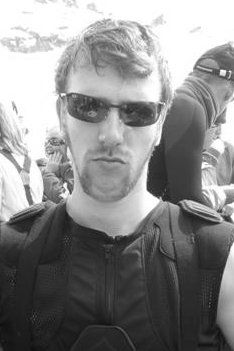
\includegraphics[width=1in,height=1.25in,clip,keepaspectratio]{anthony}}]
%{Anthony Van Herrewege} Testen maar

%Nog eentje
%\end{IEEEbiography}


% Lege achterpagina
%\clearpage
%\mbox{~}
%\thispagestyle{empty}

\end{document}
